\appendix
\clearpage{\renewcommand{\appendixname}{Anexo}

\chapter{Anexos}\label{anex}

\section{Flujo KNIME del componente AutoML Clasificacion (pre-procesado)}\label{anex:flujo-automl-componente}
\begin{figure}
	\centering
	\includegraphics[width=0.8\linewidth]{"figuras/capi 1/flujo-automl-componente"}
	\caption{Flujo KNIME del Componente AutoML Clasificación (pre-procesado) \citep{Carrazana2022}}
	\label{aped.flujo-automl-componente}
\end{figure}

\section{Flujo KNIME del procesamiento de RProp con HPO}\label{anex:flujo-hpo-rprop}
\begin{figure}[H]
	\centering
	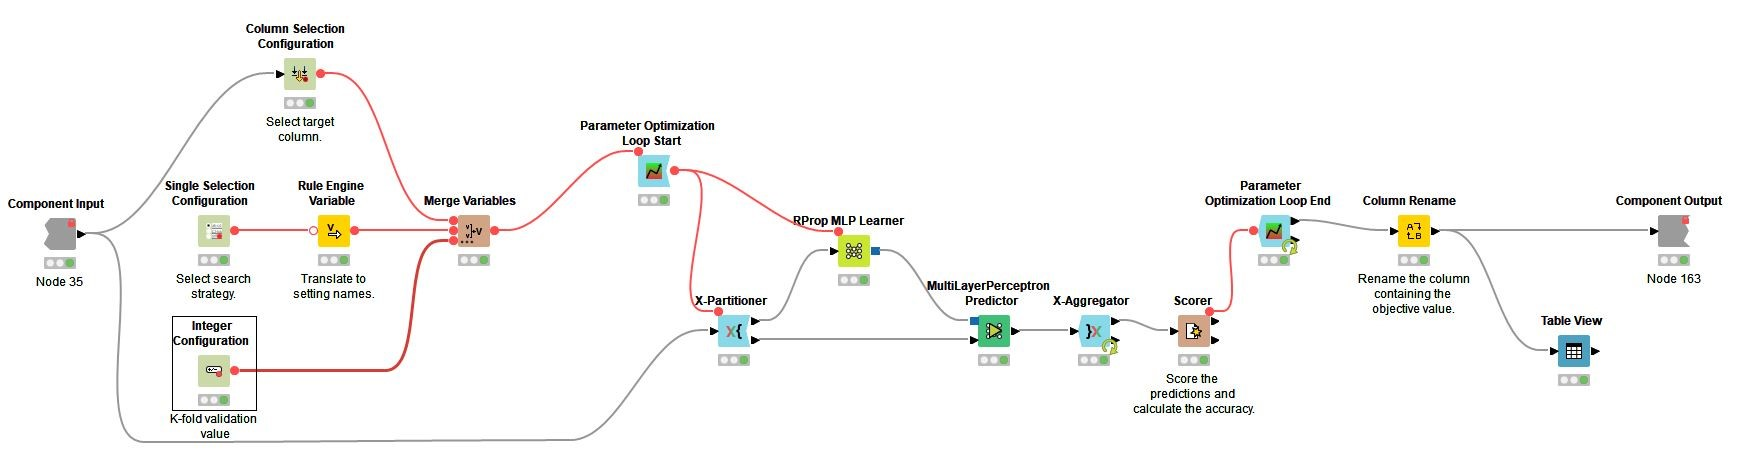
\includegraphics[width=0.9\linewidth]{figuras/anexos/flujo-hpo-rprop}
	\caption[Flujo KNIME del procesamiento de RProp con HPO]{Flujo KNIME del procesamiento de RProp con HPO}
	\label{aped.flujo-hpo-rprop}
\end{figure}

\section{Flujo KNIME de subcomponente para la discretización para el algoritmo ID3} \label{anex:flujo-disc-comp-id3}

\begin{figure}[H]
	\centering
	\includegraphics[width=0.7\linewidth]{"figuras/capi 2/diagrama-flujo-gral-disc-id3"}
	\caption{Flujo KNIME de subcomponente para la discretización para el algoritmo ID3}
	\label{fig:diagrama-flujo-gral-disc-id3}
\end{figure}

\section{Flujo KNIME de la ejecución del método CAIM para la discretización orientada al algoritmo ID3} \label{anex:flujo-discret-id3}
\begin{figure}[H]
	\centering
	\includegraphics[width=0.7\linewidth]{"figuras/capi 2/flujo-discret-id3"}
	\caption{Flujo KNIME de la ejecución del método CAIM para la discretización orientada al algoritmo ID3}
	\label{fig:flujo-discret-id3}
\end{figure}

\section{Flujo KNIME para la comparación de métodos de discretización acorde al algoritmo ID3} \label{anex:flujo-comp-alg-id3-disc}
\begin{figure}[H]
	\centering
	\includegraphics[width=0.7\linewidth]{"figuras/capi 2/flujo-comp-alg-id3-disc"}
	\caption{Flujo KNIME para la comparación de métodos de discretización acorde al algoritmo ID3}
	\label{fig:flujo-comp-alg-id3-disc}
\end{figure}

\section{Columnas de tipo String en BD3}\label{anex:bd3-tipo-dato}
\begin{figure}[H]
	\centering
	\includegraphics[width=0.4\linewidth]{"figuras/capi 3/pruebas-jenn/bd-kr_vs_kp-tipos-string"}
	\caption{Columnas de tipo String en BD3}
	\label{fig:bd-krvskp-tipos-string}
\end{figure}
